

\section{Holographic Agent Assessment Framework}
\label{sec:framework}

\subsection{Overview: Trustworthiness over a Scenario Manifold}
\label{subsec:overview}

To operationalize representative, deployment-aligned trustworthiness estimation, we introduce the \textbf{Holographic Agent Assessment Framework} (HAAF). The central idea is to move from evaluating agents on a flat collection of benchmark instances to evaluating them over a structured \emph{socio-technical scenario manifold}. The term ``holographic'' emphasizes that trustworthiness cannot be faithfully reconstructed from any single projection of behavior: reliability, robustness, safety, and alignment emerge only when an agent is examined from multiple complementary views under representative deployment conditions.

We model each scenario $s \in \mathcal{S}$ as a structured configuration that may vary along several axes, including task objective, tool interface, interaction depth, environmental constraint, social context, and consequence severity. For an agent $a$ and a scenario $s$, the framework produces a vector of trustworthiness measurements $\mathbf{m}(a,s) = (m_{P_1}(a,s), \dots, m_{P_5}(a,s))$ aligned with the five properties of Section~\ref{subsec:defining_trustworthiness}. Aggregated over a weighted test set $Q \subset \mathcal{S}$, this yields an estimated trustworthiness profile:
\[
\hat{\mathbf{T}}_{Q}(a) = \frac{1}{Z}\sum_{s \in Q} w(s)\,\mathbf{m}(a,s),
\]
where $w(s)$ encodes both deployment relevance and risk sensitivity, and $Z=\sum_{s \in Q} w(s)$ is a normalisation factor. When $w(s) \propto P_{\mathrm{deploy}}(s)$, $\hat{\mathbf{T}}_{Q}$ estimates deployment-average trustworthiness; when high-consequence scenarios are upweighted, it becomes a risk-aware assessment rather than a pure estimator of $\mathbf{T}(a)$. In our architecture, \emph{Layer~4} determines \emph{what} should be tested by generating representative scenarios and associated weights, while \emph{Layers~1--3} determine \emph{how} the agent should be probed through complementary signals and stressors. Table~\ref{tab:layer_property} summarises which properties each layer primarily probes, making explicit that no single layer is sufficient. This separation of sampling from instrumentation means the result is not a single benchmark score, but a multi-dimensional trustworthiness profile that supports coverage analysis, root-cause diagnosis, and targeted improvement. Figure~\ref{fig:framework} overviews the framework and a Factory cycle.

\begin{table}[!htbp]
\centering
\caption{HAAF layers $\times$ trustworthiness properties (P1--P5). $\bullet$~= primary probing target, $\circ$~= secondary signal. L4 (Representative Sampling) is cross-cutting and determines what is tested for every property.}
\label{tab:layer_property}
\small
\setlength{\tabcolsep}{3pt}
\begin{tabular}{@{}lccccc@{}}
\toprule
& \textbf{P1 Rel.} & \textbf{P2 Rob.} & \textbf{P3 Safe.} & \textbf{P4 S-Eth.} & \textbf{P5 Op.} \\
\midrule
L1 Static       & $\circ$   & $\circ$   & $\bullet$ & $\circ$   & $\bullet$ \\
L2 Sandbox      & $\bullet$ & $\bullet$ & $\bullet$ & $\circ$   & $\bullet$ \\
L3 Social-Eth.  & $\circ$   & $\circ$   & $\circ$   & $\bullet$ & ---       \\
\bottomrule
\end{tabular}
\end{table}

\paragraph{Failure attribution.}
HAAF attributes violated trajectories using a nine-class taxonomy---Prompt Injection (PI), Goal Drift (GD), Unauthorized Action (UA), Harmful Tool-use (HT), Resource Failure (RF), Output Failure (OF), Policy Leak (PL), Social Harm (SH), and \emph{Improper Refusal} (IR)---each mapped to one or more of P1--P5; the full mapping and definitions appear in Table~\ref{tab:taxonomy} (\S\ref{sec:experiments}). We list IR explicitly here because it is a first-class member of the taxonomy and not a residual category: IR captures cases in which the agent refuses or substantially fails to help with a \emph{benign, legitimate} request, and is mapped to P1 (Reliability) rather than to safety, so that over-refusal is correctly penalised alongside under-refusal in any deployment-relevant trustworthiness profile.

\paragraph{Comparison methodology.}
A key purpose of HAAF is to support \emph{principled comparison} between different agentic systems, not merely diagnosis of one system in isolation. Because trustworthiness is multi-dimensional (\S\ref{subsec:defining_trustworthiness}), we compare two systems $a, a'$ along three complementary views derived from their profiles. (i)~\emph{Property-wise contrast}: we report $\hat T_{P_k}(a)$ vs.\ $\hat T_{P_k}(a')$ for each $k\in\{1,\dots,5\}$, so that one system being strictly better on robustness while strictly worse on social alignment is surfaced rather than averaged away. (ii)~\emph{Pareto-dominance check}: $a$ dominates $a'$ iff $\hat T_{P_k}(a) \ge \hat T_{P_k}(a')$ for all $k$ and is strictly better on at least one; otherwise the two systems represent a trade-off that the deployment context must resolve. (iii)~\emph{Risk-weighted aggregate}: when a deployment context has known priorities $\boldsymbol{\lambda}$ over properties (e.g., regulated industries weighting P3, P4 above P1), we report the scalar $\sum_k \lambda_k \hat T_{P_k}$ as a context-conditioned summary. We deliberately do not collapse the profile to a single context-free scalar. The cross-model comparison in \S\ref{subsec:profile_comparison} instantiates this methodology over 13 contemporary agentic systems from seven model families.

\begin{figure}[!htbp]
\centering
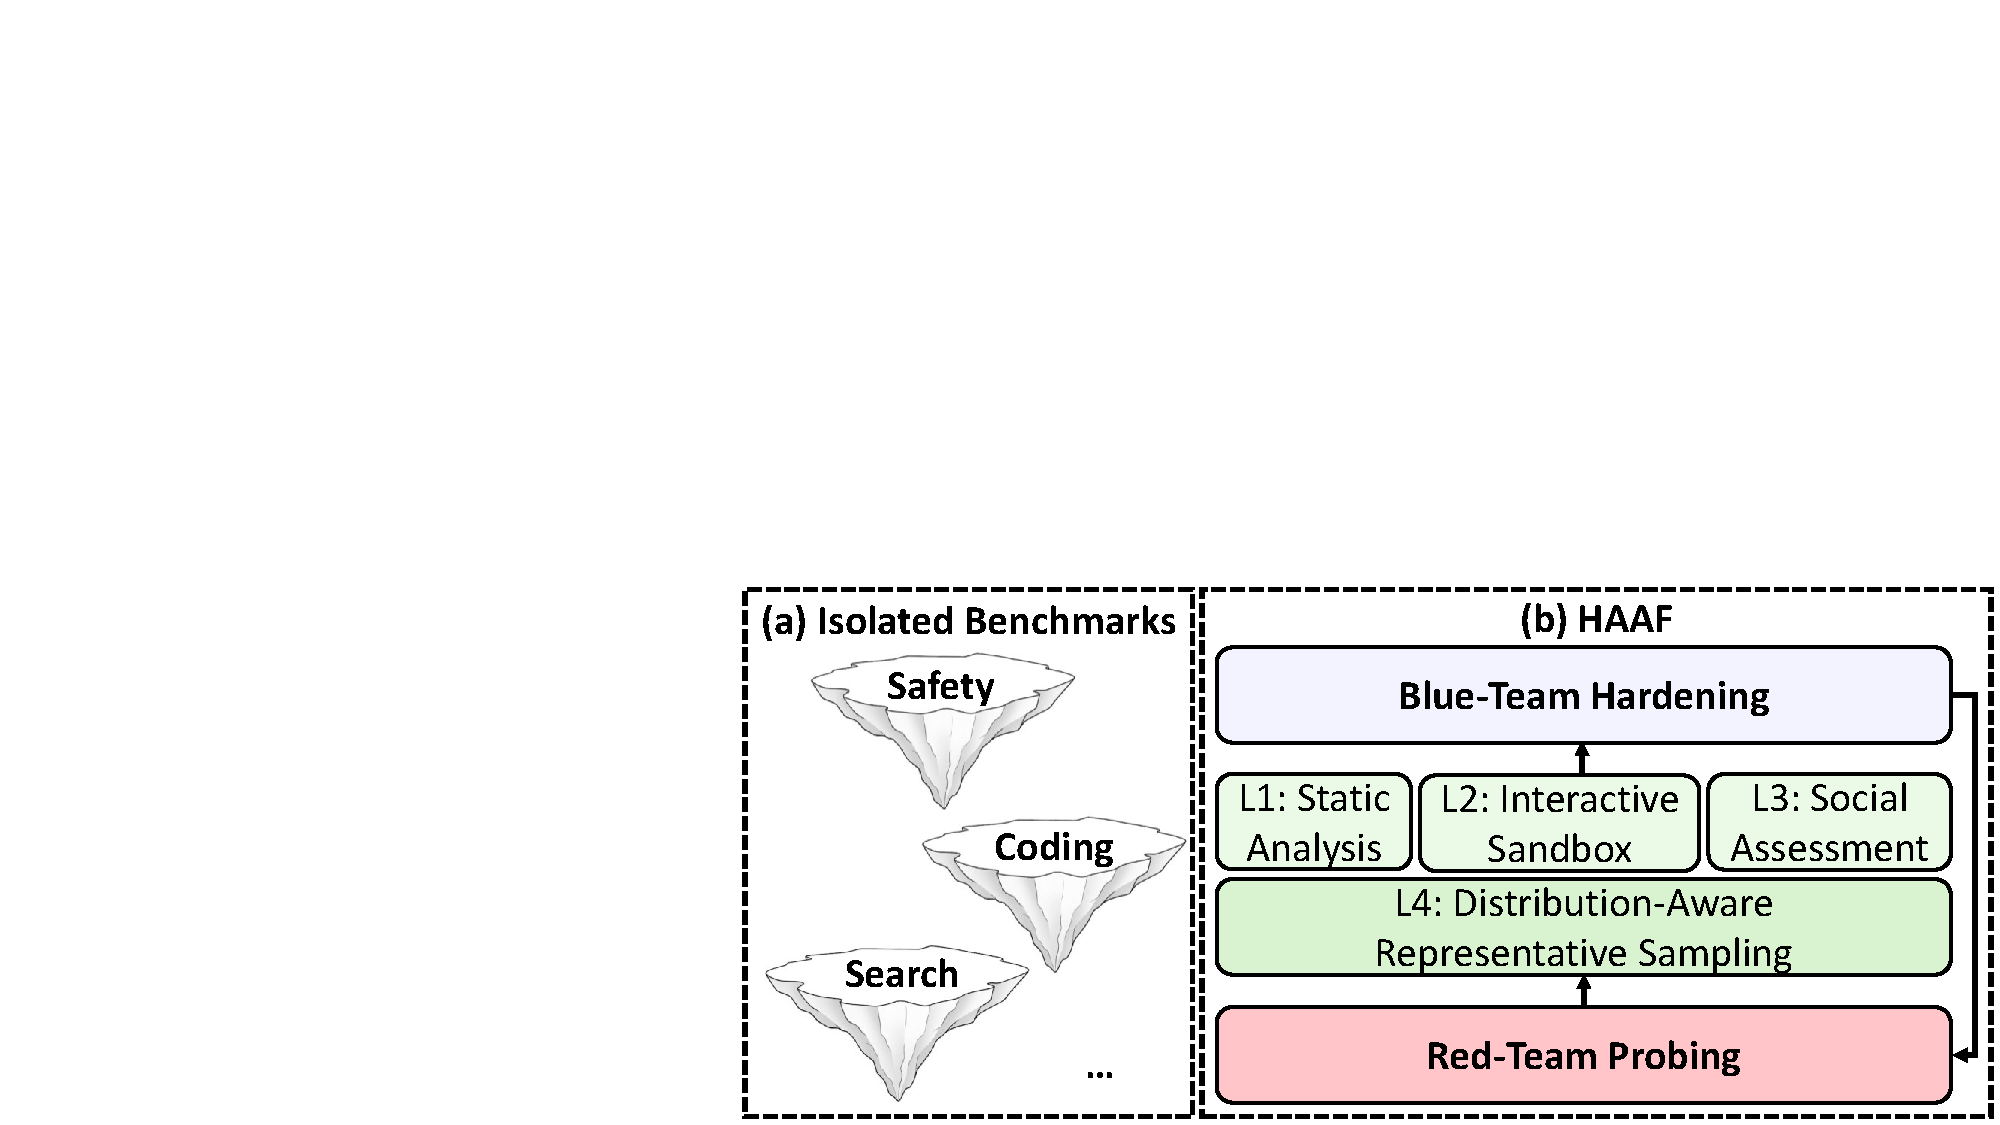
\includegraphics[width=\columnwidth,clip,trim=12cm 0cm 0cm 9.5cm]{figures/main_figure_yifan1.pdf}
\caption{\textbf{(a)}~Current benchmarks evaluate isolated capability islands (safety, coding, search, etc.) without a unified distributional perspective. \textbf{(b)}~The Holographic Agent Assessment Framework (HAAF): Layer~4 generates representative scenarios via distribution-aware sampling; Layers~1--3 probe the agent from complementary views (static analysis, interactive sandbox, and social-ethical assessment); the Trustworthy Optimization Factory iterates red-team probing and blue-team hardening until deployment readiness.}
\label{fig:framework}
\end{figure}

\subsection{Layer 1: Static Cognitive and Policy Analysis}
\label{subsec:layer1}

Layer~1 performs \emph{static cognitive and policy analysis} on \emph{policy-visible artifacts}---system instructions, tool descriptions, permission scopes, memory interfaces, retrieval sources, escalation rules, and observable decision rationales---to identify latent vulnerability surfaces before interaction begins. It probes structural issues (conflicting objectives, underspecified safety boundaries, missing confirmation barriers for irreversible operations, bias-inducing retrieval or memory) and emits a structured set of static risk hypotheses that prioritise downstream dynamic tests and distinguish mis-specified-policy failures from runtime-robustness failures.

\subsection{Layer 2: Interactive Sandbox Simulation}
\label{subsec:layer2}

Layer~2 evaluates agents through \emph{interactive sandbox simulation}~\cite{yao2024taubench,lu2024toolsandbox}, recording full trajectories (tool calls, intermediate states, deviations, recovery, downstream consequences) under three scenario classes: (i)~\emph{benign but complex tasks} for reliability under normal use; (ii)~\emph{adversarial or deceptive conditions} (prompt injection, tool-output corruption~\cite{debenedetti2024agentdojo,liu2023promptinj}) for robustness; and (iii)~\emph{resource- and environment-constrained settings} (latency, partial failure) for graceful degradation. A \emph{world model library} exposes diverse interfaces (OS, web, databases, APIs, enterprise tools).

\paragraph{Sandbox Fidelity Ladder.}
A standing objection to any sandboxed evaluation is that synthetic tools do not capture the failure modes of production systems. We make the realism dimension explicit by organising sandboxes along a four-rung \emph{Sandbox Fidelity Ladder}: \textbf{L1 Toy}---hand-authored synthetic tools over synthetic data, prioritising reproducibility and safety; \textbf{L2 Controlled}---production-like tool surfaces backed by a sandbox replica of real services (e.g., shadow databases, mock APIs with realistic schemas and latency); \textbf{L3 Shadowed-prod}---live read paths against production data with write paths shadowed to staging, so that consequences remain reversible; and \textbf{L4 Live}---agents deployed to production users with end-to-end audit logs and rollback. The instantiation in this paper is unambiguously L1, which we treat as a feature of the v1 methodology rather than a hidden limitation: the framework, the property taxonomy, the sampling objective, and the Factory cycle are invariant to which rung the sandbox sits on, and only the cost-of-error and the deployment-relevance weight $w(s)$ change as one climbs the ladder. Lifting our instantiation to L2--L3 is concrete future work (\S\ref{sec:discussion}), not a re-design.

\subsection{Layer 3: Social and Ethical Alignment Assessment}
\label{subsec:layer3}

Layer~3 extends evaluation to \emph{social and ethical alignment}~\cite{zhou2023sotopia,pan2023machiavelli}: simulated multi-party settings (human--agent collaboration, agent--agent coordination, institutional workflows, role-conditioned delegation, approval, negotiation) probe biased decisions, susceptibility to emotional or strategic manipulation, collusion, over-compliance with unsafe authority, and value drift---trustworthiness dimensions invisible to technical-only evaluations.

\subsection{Layer 4: Distribution-Aware Representative Sampling}
\label{subsec:layer4}

The core engine of HAAF is \emph{distribution-aware representative sampling}, which determines which scenarios from the manifold should be included in evaluation and with what emphasis. This layer is central because the main challenge identified in Section~\ref{sec:related_work} is not merely to test more behaviors, but to test the \emph{right distribution} of behaviors. A benchmark that samples convenient, clean, or popular instances may still fail to measure deployment trustworthiness if it omits rare but consequential events or under-represents important classes of socio-technical interaction.

We therefore treat representative evaluation as a structured sampling problem. The scenario manifold is partitioned into regions defined by dimensions such as task family, interface type, interaction horizon, environmental stress, social sensitivity, and consequence severity. For each region, the framework estimates at least two quantities: its \emph{deployment relevance}, reflecting how often similar situations arise in practice, and its \emph{risk contribution}, reflecting the cost or severity of failure when such situations occur~\cite{koh2021wilds,liang2023helm,kiela2021dynabench,shirali2022dynamicbench}. The goal is not to mirror empirical frequency alone, nor to focus only on adversarial edge cases, but to jointly account for both \emph{coverage} and \emph{risk sensitivity}.

Conceptually, the sampling objective selects a weighted scenario set $Q^{*} = \arg\max_{Q \subseteq \mathcal{S}} [\alpha\,\mathrm{Cov}(Q) + \beta\,\mathrm{Risk}(Q) + \eta\,\mathrm{Comp}(Q) - \gamma\,\mathrm{Red}(Q)]$,
where $\mathrm{Cov}(Q)$ measures manifold coverage, $\mathrm{Risk}(Q)$ emphasizes high-consequence regions, $\mathrm{Comp}(Q)$ rewards compositional diversity across co-occurring pressures, and $\mathrm{Red}(Q)$ penalizes redundant scenarios. This is not a fixed optimization recipe, but a design principle: representative evaluation should favor scenario sets that cover both frequent workflows and low-frequency high-impact failures.

A practical sampling engine can draw evidence from deployment logs, incident reports, red-team libraries, and expert-defined risk schemas, and should support \emph{compositional scenario generation} where several pressures co-occur, because many real-world failures arise from interacting stressors rather than any single one.

\subsubsection{Sampling Objective and Reference Implementation}
\label{subsubsec:layer4_reference}

To prevent the sampling objective from remaining a purely conceptual prescription, we ship a concrete reference implementation, \texttt{layer4\_\allowbreak sampling.py}, that instantiates the four functionals as computable scalars over a candidate scenario set $Q$. $\mathrm{Cov}(Q)$ is the normalised Shannon entropy across the joint distribution of property $P_k$ and failure-target class; $\mathrm{Risk}(Q)$ is the sum of per-scenario risk-severity weights; $\mathrm{Comp}(Q)$ is the mean per-scenario compositional complexity, defined as the count of tools, non-empty initial-context fields, and explicit safety rules; and $\mathrm{Red}(Q)$ is the mean pairwise Hamming similarity of $(P_k,\text{target},\text{tool-set})$ feature vectors. A greedy submodular selection with weights $(\alpha,\beta,\eta,\gamma)=(0.4,0.3,0.2,0.1)$ picks $K{=}40$ of the 100 (hand-authored) validation scenarios. Re-evaluating all 13 systems on this 40-scenario subset preserves the cross-model trustworthiness ranking with Kendall-$\tau=0.890$ and Spearman-$\rho=0.963$ (Table~\ref{tab:layer4_validation}), indicating that a $2.5\times$ smaller, objective-selected suite recovers the same comparative conclusions at substantially lower evaluation cost.

% Auto-generated by layer4_sampling.py - do not edit by hand.
\begin{table}[!htbp]
\centering
\caption{Layer-4 sampling-objective validation. The greedy submodular selection (\S\ref{subsec:layer4}) picks $K{=}40$ of $100$ scenarios under $\alpha\,\mathrm{Cov}+\beta\,\mathrm{Risk}+\eta\,\mathrm{Comp}-\gamma\,\mathrm{Red}$ with $(\alpha,\beta,\eta,\gamma)=(0.4,0.3,0.2,0.1)$. $\mathrm{RWF}_{\text{full}}$ uses all 100 scenarios; $\mathrm{RWF}_{\text{sub}}$ uses the 40 selected scenarios with the same per-model logs. Cross-model rank correlation: Kendall-$\tau=0.890$, Spearman-$\rho=0.963$.}
\label{tab:layer4_validation}
\small
\setlength{\tabcolsep}{4pt}
\begin{tabular}{lcccc}
\toprule
\textbf{System} & $\mathrm{RWF}_{\text{full}}$ & $\mathrm{RWF}_{\text{sub}}$ & $|\Delta\mathrm{RWF}|$ & $|\Delta\mathrm{rank}|$ \\
\midrule
Llama-3.1-8B & 0.216 & 0.320 & 0.104 & 0.0 \\
Llama-3.1-70B & 0.407 & 0.594 & 0.187 & 1.0 \\
Mistral-Large-2 & 0.301 & 0.457 & 0.156 & 0.0 \\
Mistral-Large-3 & 0.396 & 0.548 & 0.152 & 0.5 \\
Kimi-K2-Thinking & 0.434 & 0.624 & 0.190 & 0.0 \\
Kimi-K2.5 & 0.374 & 0.553 & 0.179 & 2.0 \\
GLM-4.7 & 0.333 & 0.497 & 0.164 & 0.0 \\
GLM-5 & 0.153 & 0.223 & 0.070 & 0.0 \\
Qwen3-32B & 0.462 & 0.675 & 0.213 & 1.0 \\
Qwen3-Next-80B & 0.587 & 0.802 & 0.215 & 0.0 \\
GPT-oss-20B & 0.418 & 0.548 & 0.130 & 2.5 \\
GPT-oss-120B & 0.481 & 0.629 & 0.149 & 1.0 \\
DeepSeek-V3.2 & 0.486 & 0.726 & 0.240 & 0.0 \\
\bottomrule
\end{tabular}
\end{table}


\subsection{The Trustworthy Optimization Factory}
\label{subsec:factory}

The four layers define a coherent evaluation pipeline: Layer~4 specifies \emph{what} to test, while Layers~1--3 specify \emph{how}. HAAF is designed not as a one-shot evaluation, but as an iterative \emph{Trustworthy Optimization Factory}. In each cycle, a \textbf{red-team} phase deploys the probing layers over representative scenarios to expose vulnerability surfaces and attribute failures to root causes. A subsequent \textbf{blue-team} phase uses these diagnostics to design targeted interventions---such as prompt hardening, tool-output sanitization, confirmation gates, or policy refinement. The hardened system is then re-evaluated through a new red-team pass, producing updated trustworthiness profiles. This cycle repeats until convergence metrics (e.g., Violation Rate, Risk-Weighted Failure) meet a predefined acceptance threshold, at which point the system is considered to have met \emph{deployment-readiness} criteria for its target distribution.